\begin{framed}
\begin{wrapfigure}{r}{0pt}
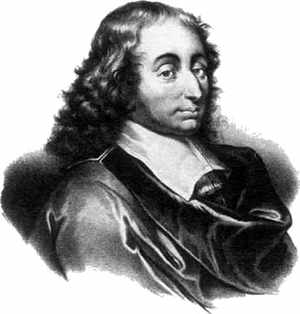
\includegraphics[width=4cm]{images/blaise_pascal.jpg}
\end{wrapfigure} 
\textbf{Blaise Pascal} ($1623-1662$)\\ French mathematician, physicist, and religious philosopher. He
was a child prodigy who already at the age of sixteen was corresponding, by letter, with the mighty Rene Descartes
($1596-1650$). When Descartes later leaned the age of Pascal he refused to believe that so young a boy was the author of
such brilliant mathematics. 

\myindent Pascal, like Newton, was a devoted theologist who spend most of his life pondering religious questions instead
of mathematical ones. By studying omens in the events around him he in fact ended up dropping mathematics completely,
since he found it apparent that God's plan for him did not include mathematics. But at the age of $35$ Pascal observed
that a particular nagging toothache seamed to go away when he pondered about mathematical things.  He concluded that
this was a good omen and thus spend one week in hectic mathematical activity. He never returned to mathematics after
this and died at the age of 39. 

\myindent Even with such a short and unfocused scientific career, Pascal managed to do become a first rate scientist. He
made important contributions to the construction of mechanical calculators, the study of fluids, and clarified the
concepts of pressure and vacuum. Pascal also helped create two major new areas of research. He wrote a significant
treatise on the subject of projective geometry and later corresponded with Pierre de Fermat on probability theory.
\end{framed}
